% ex: ts=2 sw=2 sts=2 et filetype=tex
% SPDX-License-Identifier: CC-BY-SA-4.0

\section{Introducción a HTML}

\begin{frame}[c]{¿Qué es HTML?}
  \vspace{\baselineskip}
  HTML es el lenguaje de marcado estándar para las páginas web.

  \vspace{\baselineskip}
  Con HTML puedes crear tu propio sitio web.

  \vspace{\baselineskip}
  HTML es fácil de aprender - ¡Lo disfrutarás!
\end{frame}

\begin{frame}[c]{¿Qué es HTML?}
  \begin{itemize}
    \item HTML significa Lenguaje de Marcado de HiperTexto
    \pausa
    \item HTML es el lenguaje de marcado estándar para crear páginas web.
    \pausa
    \item HTML describe la estructura de una página Web
    \pausa
    \item HTML consta de una serie de elementos
    \pausa
    \item Los elementos HTML le dicen al navegador cómo mostrar el contenido
    \pausa
    \item Los elementos HTML etiquetan piezas de contenido como
      "este es un encabezado", "este es un párrafo", "este es un enlace", etc.
  \end{itemize}
\end{frame}

\begin{frame}[fragile]
  \frametitle{Un documento HTML simple}
  \lstinputlisting{ejemplo01.html}
\end{frame}

\begin{frame}[c]{Ejemplo explicado}
  \begin{itemize}
    \item La declaración \textcolor{blue}{<!DOCTYPE} html\textcolor{blue}{>}
      define que este documento es un documento HTML5
    \pausa
    \item El elemento \textcolor{blue}{<html>} es el elemento raíz
      de una página HTML
    \pausa
    \item El elemento \textcolor{blue}{<head>} contiene metainformación
      sobre la página HTML
    \pausa
    \item El elemento \textcolor{blue}{<title>} especifica un título para
      la página HTML (que se muestra en la barra de título del navegador o
      en la pestaña de la página)
    \pausa
    \item El elemento \textcolor{blue}{<body>} define el cuerpo del
      documento y es un contenedor de todos los contenidos visibles, como
      encabezados, párrafos, imágenes, hipervínculos, tablas, listas, etc.
    \pausa
    \item El elemento \textcolor{blue}{<h1>} define un encabezado grande
    \pausa
    \item El elemento \textcolor{blue}{<p>} define un párrafo
  \end{itemize}
\end{frame}


\begin{frame}[c]{¿Qué es un elemento HTML?}

  Un elemento HTML se define mediante una \textbf{etiqueta} de inicio,
  algo de contenido y una \textbf{etiqueta} de finalización:

  \vspace{\baselineskip}
  \textcolor{blue}{<nombre\_de\_la\_etiqueta>} el contenido va aquí
  \textcolor{blue}{</nombre\_de\_la\_etiqueta>}

  \pausa
  \vspace{\baselineskip}
  El elemento HTML es todo, desde la etiqueta de inicio hasta la
  etiqueta final:

  \vspace{\baselineskip}
  \textcolor{blue}{<h1>}Mi primer encabezado\textcolor{blue}{</h1>}

  \vspace{\baselineskip}
  \textcolor{blue}{<p>}Mi primer párrafo.\textcolor{blue}{</p>}

  \begin{exampleblock}{Nota:}
    La etiqueta final siempre tiene una / al inicio.
  \end{exampleblock}

\end{frame}


\begin{frame}[c]{¿Qué es un elemento HTML?}

  \begin{table}[]
  \begin{tabular}{cll}
    \textbf{Etiqueta de inicio} &  \textbf{Contenido del elemento} & \textbf{Etiqueta final} \\
    \rowcolor{light-gray}
    <h1>& Mi primer encabezado & </h1> \\
    <p>& Mi primer párrafo.& </p> \\
    \rowcolor{light-gray}
    <br>&  nada & nada \\
  \end{tabular}
  \end{table}

  \begin{alertblock}{Nota:}
    Algunos elementos HTML no tienen contenido (como el elemento <br>).
    Estos elementos se denominan elementos vacíos. ¡Los elementos vacíos
    no tienen una etiqueta final!
  \end{alertblock}
\end{frame}

\begin{frame}[c]{Navegadores web}

  El propósito de un navegador web (Chrome, Edge, Firefox, Safari)
  es leer documentos HTML y mostrarlos correctamente.

  \vspace{\baselineskip}
  Un navegador no muestra las etiquetas HTML, pero las usa para
  determinar cómo mostrar el documento
\end{frame}

\begin{frame}[c]{Estructura de una página HTML}
  \begin{columns}
    \column{0.4\textwidth}
      A continuación se muestra una visualización de la
      estructura de una página HTML:

      \begin{exampleblock}{Nota:}
        El contenido dentro de la sección <body> (el área blanca ) se
        mostrará en un navegador. El contenido dentro del elemento <title>
        se mostrará en la barra de título del navegador o en la pestaña de
        la página.
      \end{exampleblock}

    \column{0.6\textwidth}
      \begin{center}
        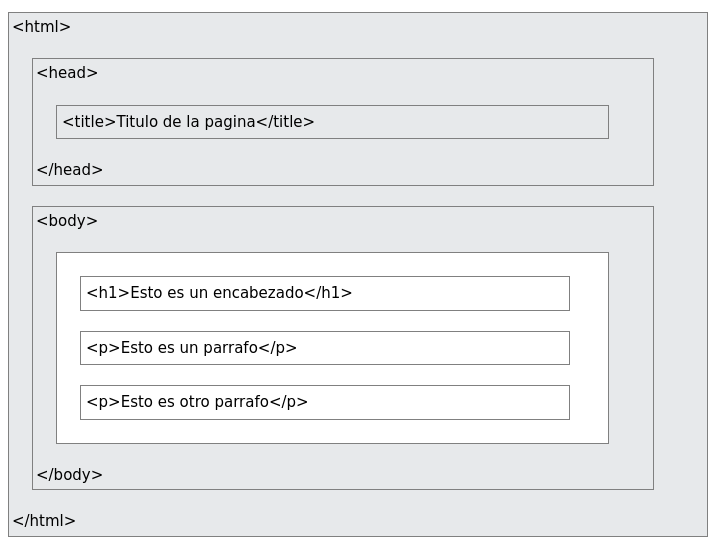
\includegraphics[scale=0.35]{01-estructura-html.png}
      \end{center}
  \end{columns}
\end{frame}

\begin{frame}[c]{Historia del HTML}
  \begin{table}[]
  \begin{tabular}{cll}
    \textbf{Año} &  \textbf{Versión} \\
    \rowcolor{light-gray}
    1989 & Tim Berners-Lee inventó www \\
    1991 & Tim Berners-Lee inventó HTML \\
    \rowcolor{light-gray}
    1993 & Dave Raggett redactó HTML+ \\
    1995 & el Grupo de trabajo HTML definido HTML 2.0 \\
    \rowcolor{light-gray}
    1997 & Recomendación del W3C: HTML 3.2 \\
    1999 & Recomendación del W3C: HTML 4.01 \\
    \rowcolor{light-gray}
    2000 & Recomendación W3C: XHTML 1.0 \\
    2008 & WHATWG HTML5 Primer borrador público \\
    \rowcolor{light-gray}
    2012 & WHATWG HTML5 Estándar de vida \\
    2014 & Recomendación W3C: HTML5 \\
    \rowcolor{light-gray}
    2016 & Candidato a recomendación del W3C: HTML 5.1 \\
    2017 & Recomendación W3C: HTML5.1 2da edición \\
    \rowcolor{light-gray}
    2017 & Recomendación W3C: HTML5.2 \\
  \end{tabular}
  \end{table}
\end{frame}

\begin{frame}[c]{Historia del HTML}
  Como vimos, desde los primeros días de la World Wide Web,
  ha habido muchas versiones de HTML.

  \vspace{\baselineskip}
  \begin{exampleblock}{Nota:}
    Este curso sigue el último estándar HTML5.
  \end{exampleblock}

\end{frame}

\section{Editores de HTML}

\begin{frame}[c]{Editores de texto}
  Las páginas web se pueden crear y modificar utilizando editores HTML profesionales.

  \vspace{\baselineskip}
  Sin embargo, para aprender HTML recomendamos un editor de texto simple
  como Notepad (PC) o TextEdit (Mac). De igual forma existen editores de
  texto los cuales colorean el texto.

  \vspace{\baselineskip}
  Usar un editor de texto simple es una buena manera de aprender HTML.
\end{frame}


\begin{frame}[c]{Notepad++}
  Notepad++ es un editor de texto y de código fuente libre con soporte
  para varios lenguajes de programación. Con soporte nativo para
  Microsoft Windows.

  \vspace{\baselineskip}
  Se parece al Bloc de notas en cuanto al hecho de que puede editar texto
  sin formato y de forma simple. No obstante, incluye opciones más
  avanzadas que pueden ser útiles para usuarios avanzados como
  desarrolladores y programadores.

  \vspace{\baselineskip}
  Se distribuye bajo los términos de la licencia GPLv3.

  \vspace{\baselineskip}
  \href{https://notepad-plus-plus.org/}{https://notepad-plus-plus.org/}
\end{frame}

\section{Ejemplos básicos}

\begin{frame}[c]{Ejemplos básicos}

  \vspace{\baselineskip}
  En lo siguiente mostraremos algunos ejemplos básicos de HTML.

  \vspace{\baselineskip}
  No te preocupes si usamos etiquetas que aún no conoces.
\end{frame}

\begin{frame}[c]{Documentos HTML}

  Todos los documentos HTML deben comenzar con una declaración de
  tipo de documento: \textcolor{blue}{<!DOCTYPE} html\textcolor{blue}{>}.

  \vspace{\baselineskip}
  El documento HTML en sí comienza con \textcolor{blue}{<html>} y
  termina con \textcolor{blue}{</html>}.

  \vspace{\baselineskip}
  La parte visible del documento HTML está entre \textcolor{blue}{<body>}
  y \textcolor{blue}{</body>}.
\end{frame}

\begin{frame}[fragile]
  \frametitle{Ejemplo de un documento HTML simple}
  \lstinputlisting{ejemplo02.html}
\end{frame}

\begin{frame}[fragile]
  \frametitle{La Declaración <!DOCTYPE>}

  La declaración \textbf{<!DOCTYPE>} representa el tipo de documento
  y ayuda a los navegadores a mostrar correctamente las páginas web.

  Solo debe aparecer una vez, en la parte superior de la página
  antes de cualquier etiqueta HTML).

  La declaración \textbf{<!DOCTYPE>} no distingue entre mayúsculas
  y minúsculas.

  La declaración \textbf{<!DOCTYPE>} para HTML5 es:

  \vspace{\baselineskip}
  \begin{lstlisting}
<!DOCTYPE html>
  \end{lstlisting}
\end{frame}

\begin{frame}[fragile]
  \frametitle{Encabezados HTML}

  Los encabezados HTML se definen con las etiquetas \textbf{<h1>} a
  \textbf{<h6>}.

  \textbf{<h1>} define el encabezado más importante.
  \textbf{<h6>} define el encabezado menos importante:

  \vspace{\baselineskip}
  \begin{lstlisting}
<h1>Este es el encabezado 1</h1>
<h2>Este es el encabezado 2</h2>
<h3>Este es el encabezado 3</h3>
  \end{lstlisting}
\end{frame}

\begin{frame}[fragile]
  \frametitle{Párrafos HTML}

  Los párrafos HTML se definen con la etiqueta \textbf{<p>}:

  \vspace{\baselineskip}
  \begin{lstlisting}
<p>Este es un párrafo</p>
<p>Este es otro párrafo</p>
  \end{lstlisting}
\end{frame}

\begin{frame}[fragile]
  \frametitle{Enlaces HTML}

  Los enlaces (ligas) HTML se definen con la etiqueta \textbf{<a>}:

  \vspace{\baselineskip}
  \begin{lstlisting}
<a href="https://www.google.com"> Esta es una liga </a>
  \end{lstlisting}

  \vspace{\baselineskip}
  El destino del enlace se especifica en el atributo
  \textcolor{editorGreen}{href}.

  \vspace{\baselineskip}
  Los atributos se utilizan para proporcionar información
  adicional sobre los elementos HTML.

  \vspace{\baselineskip}
  Aprenderemos más sobre los atributos en un capítulo posterior.
\end{frame}

\begin{frame}[fragile]
  \frametitle{Imágenes HTML}

  Las imágenes HTML se definen con la etiqueta \textbf{<img>}.

  El archivo de origen (\textcolor{editorGreen}{src}), el texto
  alternativo (\textcolor{editorGreen}{alt}), el ancho
  (\textcolor{editorGreen}{width}) y el alto
  (\textcolor{editorGreen}{height}) se proporcionan como atributos:

  \vspace{\baselineskip}
  \begin{lstlisting}
<img src="imagen.jpg" alt="texto alternativo" width="104" height="142">
  \end{lstlisting}
\end{frame}

\begin{frame}[c]{¿Cómo ver el código fuente HTML?}

  Alguna vez has visto una página web y te has preguntado
  "¡Oye! ¿Cómo hicieron eso?"

  \begin{block}{Ver código fuente HTML:}
    Haga clic derecho en una página HTML y seleccione "Ver código fuente"
    (en Chrome) o "Ver código fuente" (en Edge), o similar en otros
    navegadores. Esto abrirá una ventana que contiene el código fuente
    HTML de la página.
  \end{block}

  \begin{exampleblock}{Inspeccionar un elemento HTML:}
    Haga clic con el botón derecho en un elemento (o en un área en blanco)
    y elija "Inspeccionar" o "Inspeccionar elemento" para ver de qué están
    compuestos los elementos (verá tanto el HTML como el CSS). También
    puede editar HTML o CSS sobre la marcha en el panel Elementos o
    Estilos que se abren.
  \end{exampleblock}
\end{frame}

